\begin{frame}{What is this thesis about?}
\begin{block}{}
\begin{itemize}
\item A sparsely sampled light field reconstruction method of a static scene. 

\bigskip
\pause
\item This method uses Universal Shearlets to perform an inpainting algorithm in the sparse Epipolar planes images (EPIs).

\bigskip 
\pause
\item The EPIs are images with linear structures obtained by tracking different feature points in a sequence of pictures of the scene. 

\bigskip
\pause
\item The slope of the straight lines in the EPIs can be used to compute the depth of feature points in the scene and therefore the depth map that contains the 3D information of the scene.

\bigskip
\pause
\item The thesis presents all the steps in the reconstruction pipeline with theory, algorithms and code. 
\end{itemize} 
\end{block}
\end{frame}

\begin{frame}{Involved concepts}
\begin{block}{}
\begin{itemize}
\item Early Vision (biology) and Light Field Theory (physics).

\bigskip
\pause
\item Computer Vision for point tracking and line detection (basic concepts of linear algebra).

\bigskip 
\pause
\item Functional Analysis and Computational Harmonic Analysis (sparsifying dictionaries).

\bigskip
\pause
\item Compressed sensing techniques ($\ell^1$ optimization algorithms for inverse problems). 
\end{itemize}
\end{block}
\end{frame}

\begin{frame}{Light Field Theory}
\begin{block}{}
\begin{itemize}

\item In 1846 Michael Faraday proposed for the first time on his lecture "Thoughts on Ray Vibration" that light could be interpreted as a field.

\pause

\item Propagation of light rays in the 3D space is completely described by a 7D continuous function $L:\mathbb{R}^7\longrightarrow \mathbb{R}^3$, $L(x,y,z,\theta,\phi, \lambda, \tau)$ called the plenoptic function

\pause
\begin{figure}[h!]
\centering
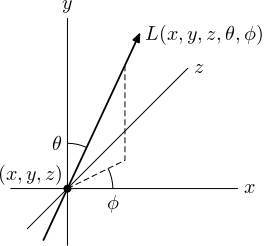
\includegraphics[width=0.3\textwidth]{../../Diagrams/Plenoptic_function.jpg}
\end{figure}

\pause

\item The plenoptic function can be simplified to a 4D function $L_4$, called 4D Light Field or simply Light Field, which quantifies the intensity of static and monochromatic light rays propagating in half space. 
\end{itemize}
\end{block}
\end{frame}

\begin{frame}{4D Light Field Representation}
\begin{figure}[h!]
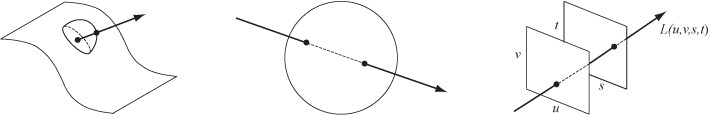
\includegraphics[width=0.8\textwidth]{../../Diagrams/Light-field-parametrizations.jpg}
\caption{Three different representation of 4F LF\@. Left: $L_4(u,v,\phi,\theta)$. Center: $L_4(\phi_1,\theta_1,\phi_2,\theta_2)$. Right: $L_4(u,v,s,t)$.}
\end{figure}
\pause
\begin{figure}[h!]
\centering
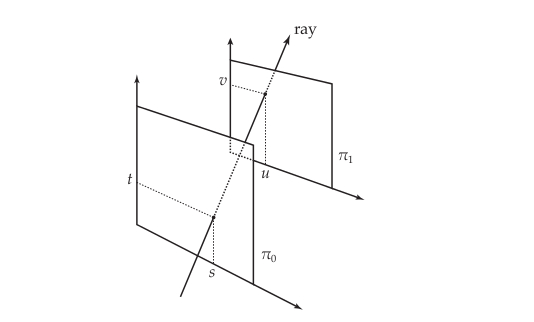
\includegraphics[width=0.5\textwidth]{../../Diagrams/two-planes_param.jpg}
\caption{Used representation: "Two plane parametrization".}
\label{fig:C2S0F3}
\end{figure}
\end{frame}

\begin{frame}{Freedom of knowledge and reproducible research}

\begin{quote}
An article about computational result is \\
advertising, not scholarship. The actual \\
scholarship is the full software environment,\\
code and data, that produced the result.
\end{quote}
\begin{flushright}
\textbf{Buckheit and Donoho (1995)}
\end{flushright}
\end{frame}

\begin{frame}{Stereo Vision and Epipolar Geometry}
\begin{block}{}
\begin{itemize}
\item \textbf{Stereo Vision:} The human brain generates the 3D depth perception of its sorroundings by triangulating the points of a scene using the information coming from both eyes.

\pause
\item \textbf{Epipolar Geometry:} Generalization of Stereo Vision with more than two views, assuming the epipolar constraint.

\pause
\item \textbf{Epipolar Constraint:} Analysis of object position while assuming the knowledge of the camera motion.
\pause
\begin{figure}[h!]
\centering
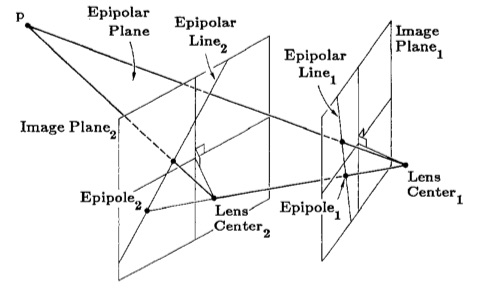
\includegraphics[width=0.52\textwidth]{../../Diagrams/epipolarline.jpg}
\end{figure}
 
\end{itemize}
\end{block}
\end{frame}

\begin{frame}{Epipolar Plane Images (EPIs) on Straight Line Trajectories}
\begin{figure}[h!]
\centering
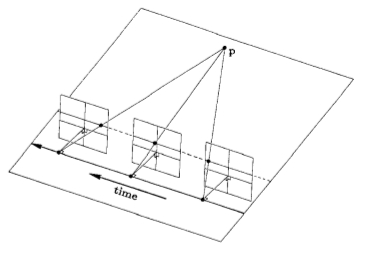
\includegraphics[width=0.45\textwidth]{../../Diagrams/perp-move.jpg}
\end{figure}

\pause
\begin{figure}[h!]
\centering
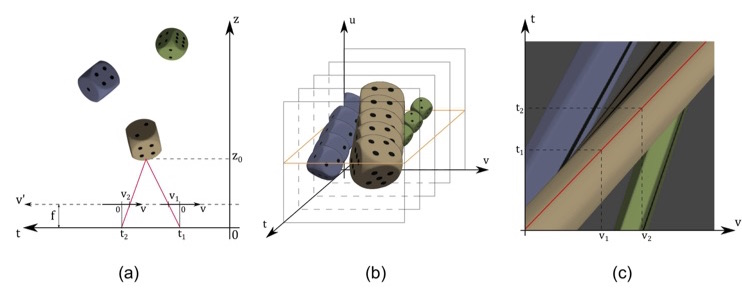
\includegraphics[width=0.90\textwidth]{../../Diagrams/EPI-dices.jpg}
\end{figure}

\end{frame}

\begin{frame}{Depth map Estimation with EPIs}
\begin{block}{}
\begin{figure}[h!]
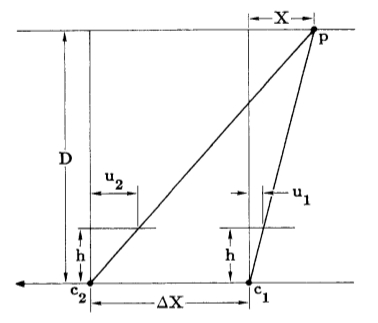
\includegraphics[width=0.5\textwidth]{../../Diagrams/stereo-dist.jpg}
\end{figure}
\pause
\begin{itemize}
\item \textbf{Point-depth formula:} $D= h\frac{\Delta X}{\Delta u}=h\frac{\Delta X}{u1-u2}$.
\pause
\item \textbf{Sampling rate (Nyquist criterion):} $\Delta X\leq \frac{D_{min}}{h}\Delta u$.
\end{itemize}
\end{block}
\end{frame}

\begin{frame}{Physical Acquisition Setup}
\begin{block}{}
\begin{itemize}
\item \textbf{Data set:} Sequence of 101 rectified pictures of a scene generated by Professor Markus Gross' group in the Disney Research Center at Zurich.
\pause
\item \textbf{Technical details of physical setup:} Canon EOS 4D Mark II DSLR camera, Canon EF 50 mm f/1.4 USM lens and a Zaber T-LST1500D motorized linear stage to drive the camera to the shooting positions with 10 mm of distance between each other. 
\pause
\begin{figure}[h!]
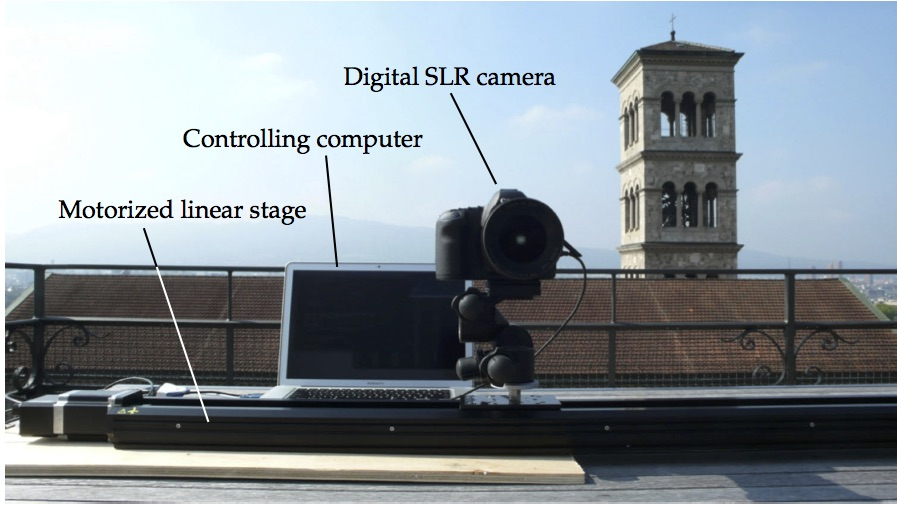
\includegraphics[width=0.6\textwidth]{../../Diagrams/setting.jpg}
\end{figure}
\end{itemize}
\end{block}
\end{frame}

\begin{frame}{Used Data Set: Church}
\begin{figure}[!tbp]
  \centering
  \begin{minipage}[b]{0.49\textwidth}
    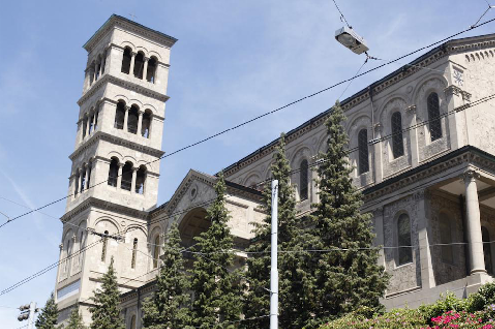
\includegraphics[width=\textwidth]{../../Diagrams/first_frame_church.png}
  \end{minipage}
	\pause
 % \hfill
  \begin{minipage}[b]{0.5\textwidth}
    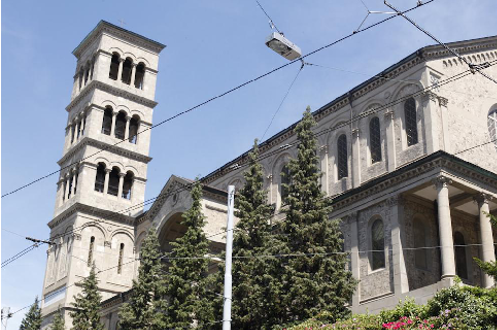
\includegraphics[width=\textwidth]{../../Diagrams/last_frame_church.png}
  \end{minipage}
\end{figure}
\end{frame}

\begin{frame}{Followed Pipeline}
\begin{block}{}
\begin{figure}[h!]
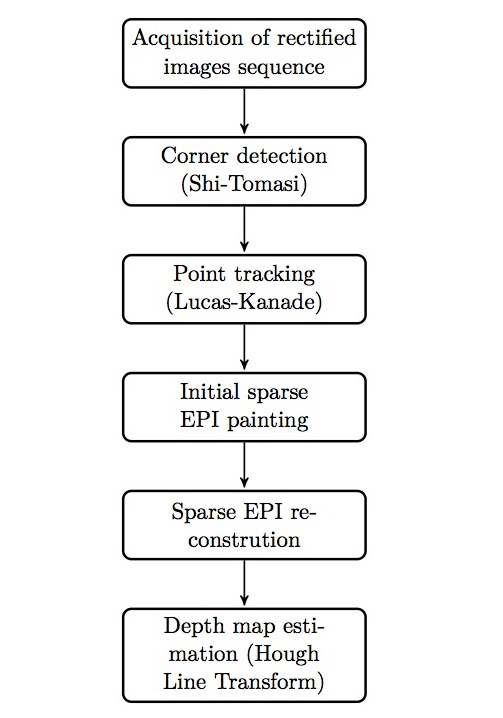
\includegraphics[width=0.4\textwidth]{./images/pipeline.jpg}
\end{figure}
\end{block}
\end{frame}

\begin{frame}{Point Tracking Results}
\begin{figure}[!tbp]
  \centering
  \begin{minipage}[b]{0.49\textwidth}
    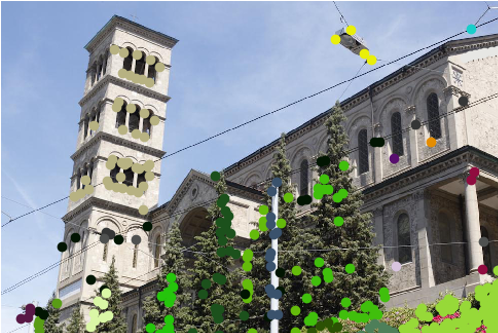
\includegraphics[width=\textwidth]{../../Diagrams/first_frame_church_points.png}
  \end{minipage}
	\pause
 % \hfill
  \begin{minipage}[b]{0.5\textwidth}
    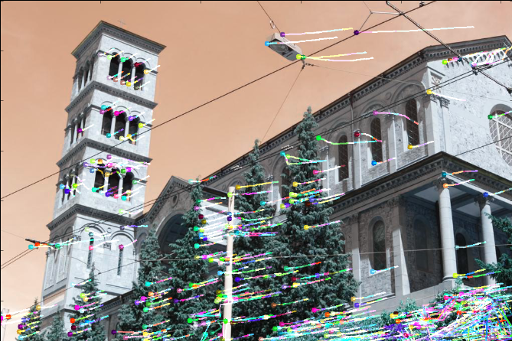
\includegraphics[width=\textwidth]{../../Diagrams/track_points_church.png}
  \end{minipage}
\end{figure}
\end{frame}

\begin{frame}{Particular EPI Example}
\begin{figure}[h!]
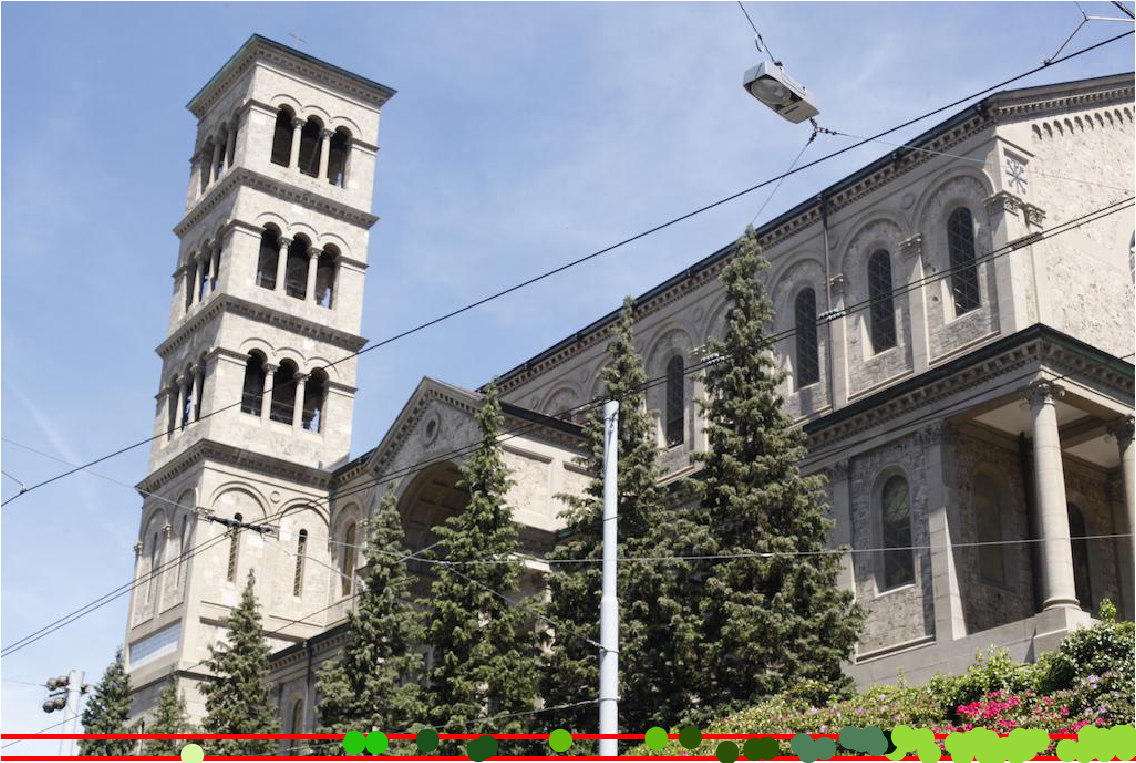
\includegraphics[width=0.45\textwidth]{../../EPIs_strips/EPIs/673_10_102_4_48_8_strip.png}
\end{figure}
\pause
\begin{figure}[!tbp]
  \centering
  \begin{minipage}[b]{0.45\textwidth}
    
\includegraphics[width=\textwidth]{../../EPIs_strips/EPIs/673_10_102_4_48_8_dense.png}
  \end{minipage}
	\pause
 % \hfill
  \begin{minipage}[b]{0.45\textwidth}
    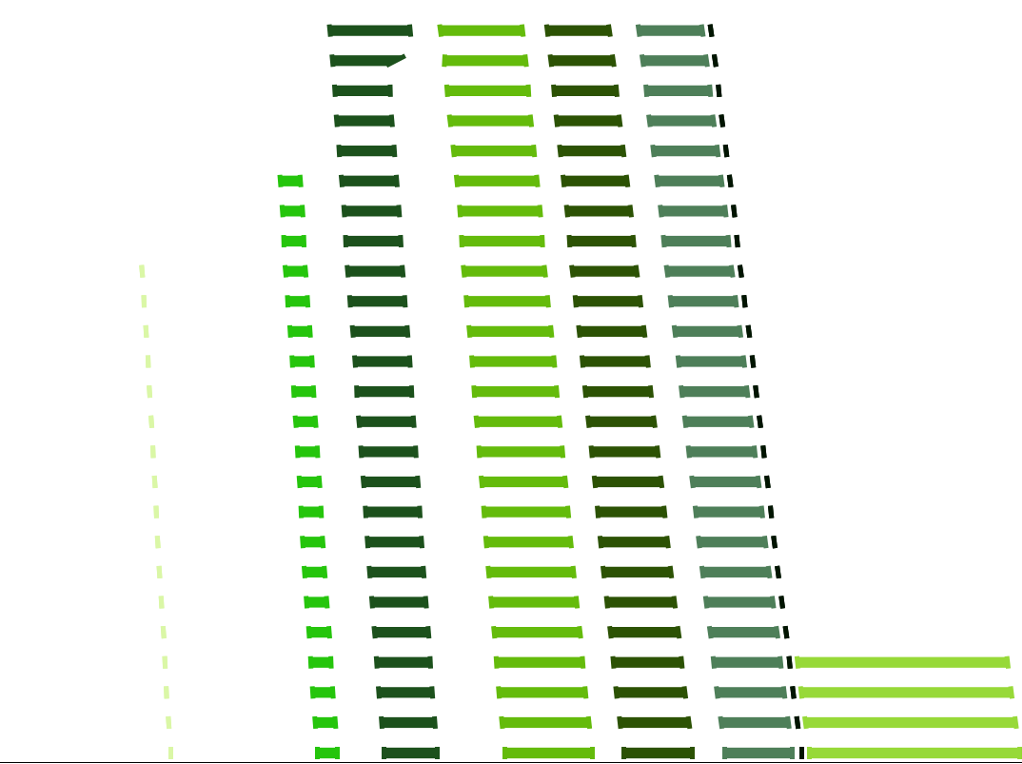
\includegraphics[width=\textwidth]{../../EPIs_strips/EPIs/673_10_102_4_48_8_sparse.png}
  \end{minipage}
\end{figure}

\end{frame}

\begin{frame}{Reconstruction Method with Inpaiting}
\begin{block}{}
\begin{figure}[h!]
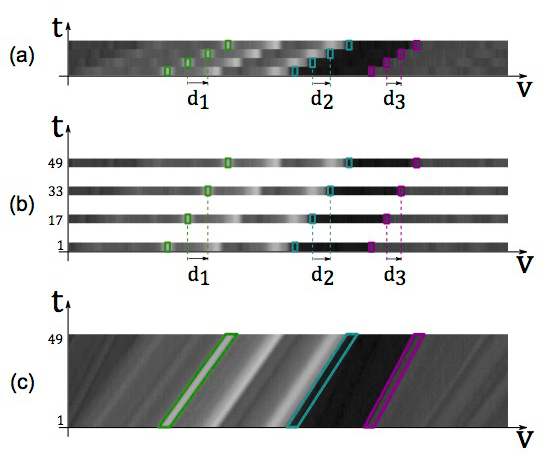
\includegraphics[width=0.7\textwidth]{../../Diagrams/sparse_EPI.jpg}
\end{figure}
\end{block}
\end{frame}

\begin{frame}{Important Tool: Frame Theory}
\begin{block}{Frames}
Let $I$ be a set of countable indices. A sequence $(\phi_i)_{i\in I}$ in a Hilbert space $\mathcal{H}$ is called a \textbf{frame} of $H$, if there exist constants $0< A\leq B<\infty$ such that
$$
A||x||^2\leq\sum_{i\in I}|\langle x,\phi_i\rangle|^2\leq B||x||^2 \text{  ,  } \forall x\in\mathcal{H}
$$
$A$ and $B$ are called lower and upper frame bound. Moreover, if $A$ and $B$ can be chosen to be equal, we call it $(A-)$tight frame. If $A=B=1$ is possible, $(\phi_i)_{i\in I}$ forms a Parseval frame. A frame $(\phi_i)_{i\in I}$ span $\mathcal{H}$. 
\end{block}
\end{frame}

\begin{frame}
\begin{block}{Analysis, synthesis and frame operator}
$T:\mathcal{H}\longrightarrow\ell_2(I)$ given by $f\mapsto (\langle f,\phi_i\rangle )_{i\in I}$ is called \textbf{the analysis operator}, and $T^*:\ell_2(I)\longrightarrow\mathcal{H}$, given by $(c_i)_{i\in I}\mapsto \sum_{i\in I}c_i\phi_i$ is called \textbf{the synthesis operator}.

$S=T^*T:\mathcal{H}\longrightarrow \mathcal{H}$, given by $f\mapsto \sum_{i\in I}\langle f,\phi_i\rangle \phi_i$ is called \textbf{the frame operator} and is an ivertible operator. 
\end{block}

\pause
\begin{block}{Reconstruction and Decompostion Formula}
If $(\phi_i)_{i\in I}\subseteq \mathcal{H}$ be a frame for $\mathcal{H}$, and $S$ its frame operator, then
$$
\begin{aligned}
f &=\sum_{i\in I}\langle f,\phi_i\rangle S^{-1}\phi_i \text{,  }\forall f\in\mathcal{H}\text{(Reconstruction)}\\
f &=\sum_{i\in I}\langle f,S^{-1}\phi_i\rangle\phi_i \text{,  }\forall f\in\mathcal{H}\text{(Decomposition)}
\end{aligned}
$$
\end{block}
\end{frame}

\begin{frame}{Abstract Inpainting Framework}
\begin{block}{}
\begin{itemize}
\item Let $\mathcal{H}$ a separable Hilbert space and $x^0\in\mathcal{H}=\mathcal{H}_K\oplus\mathcal{H}_M=P_K\mathcal{H}\oplus P_M\mathcal{H}$. Then, given a corrupt signal $P_K x^0$, we want to recover the missing part $P_Mx^0$.
\bigskip
\pause
\item In image inpanting $\mathcal{H}=L^2(\mathbb{R}^2)$, the missing space $H_M=L^2(\mathcal{M})$ for some measurable set $\mathcal{M}\subset \mathbb{R}^2$. Given $x_k\in \mathcal{H}_K$ we want to find $x^0\in\mathcal{H}$ such that $x_K=P_Kx^0$ (underdetermined problem).
\bigskip
\pause
\item We will assume that $x^0$ can be efficiently represented by some Parseval frame $\Phi=(\phi_i)_{i\in I}$ for $\mathcal{H}$, the inpainting will be translated as asking for the solution of the $\ell^0-$minimization problem
$$
\underset{c\in\ell^2(I)}{\min}||c||_{\ell^0(I)}\quad\textrm{subject to}\quad P_K x^0=P_KT_{\Phi}^*c=\sum_{i\in I}c_iP_K\phi_i
$$
\end{itemize}
\end{block}
\end{frame}

\begin{frame}{Analysis approach}
\begin{block}{}
\begin{algorithm2e}[H]
    \SetKwInOut{Input}{Input}
    \SetKwInOut{Output}{Output}
		\SetKwInOut{Compute}{Compute}

    \Input{Corrupted signal $P_Kx^0\in\mathcal{H}_K$, Parseval frame $\Phi=(\phi_i)_{i\in I}$ for $\mathcal{H}$}
		\Compute{\begin{equation}
			x^*=\underset{x\in\mathcal{H}}{\text{argmin}}||T_{\Phi}x||_{\ell^1(I)} \quad\textrm{subject to}\quad P_Kx^*=P_Kx^0=x_K
			\tag{$\ell^1-\text{INP}$}
		\end{equation}}
    \Output{recovered signal $x^*\in\mathcal{H}$}
    \caption{Inpainting via $\ell^1$-minimization}
\end{algorithm2e}
\end{block}

\pause

\begin{block}{Best N-term approx.\ error (Donoho, 2001)}
Let $\{\psi_{\lambda}\}_{\lambda\in\Lambda}\subseteq L^2(\mathbb{R}^2)$ a frame. The optimal best $N$-term approximation error for any $f\in \mathcal{E}^2(\mathbb{R}^2)$ (cartoon-like functions space) is 
$$
\sigma_N(f,\{\psi_{\lambda}\}_{\lambda\in\Lambda})=O(N^{-1})
$$
In the case of 2D-wavelets
$$
\sigma_{N}(f,\{\psi_{j,m}\}_{j,m})\sim N^{-1/2}
$$
\end{block}
\end{frame}

\begin{frame}{Shearlets}
\begin{block}{Discrete Shearlet System}
For $j\in\mathbb{Z}$, let 
$$
A_j:=\left(\begin{matrix} 2^j & 0 \\ 0 & 2^{j/2} \end{matrix}\right)
$$
be the \textbf{parabolic scaling matrix}, and for $k\in\mathbb{Z}$, let 
$$
S_k:=\left(\begin{matrix} 1 & k \\ 0 & 1\end{matrix}\right)
$$
be the \textbf{shearing matrix}. Given $\psi\in\L^2(\mathbb{R}^2)$, the \textbf{shearlet system} associated with $\psi$ is defined as 
$$
\mathcal{SH}(\psi):=\{ 2^{3j/4}\psi(S_kA_jx-m) : j\in \mathbb{Z},k\in\mathbb{Z},m\in\mathbb{Z}^2\}
$$
\end{block}
\pause
\begin{block}{Discrete Shearlet Transform}
For $f\in L^2(\mathbb{R}^2)$ the associated \textbf{discrete shearlet transform} is defined by 
$$
f\mapsto \mathcal{SH}_{\psi}f(j,k,m)=\langle f,\psi_{j,k,m}\rangle\text{,  }(j,k,m)\in\mathbb{Z}\times\mathbb{Z}\times\mathbb{Z}^2
$$
\end{block}
\end{frame}

\begin{frame}
\begin{block}{Classical Shearlets}
Let $\psi\in L^2(\mathbb{R}^2)$ defined by $\hat{\psi}(\xi_1,\xi_2)=\hat{\psi}_1(\xi_1)\hat{\psi}_2(\xi_2/\xi_1)$, where $\psi_1,\psi_2\in L^2(\mathbb{R}^2)$ satisfy the following properties:
\begin{itemize}
\item $\sum_{j\in\mathbb{Z}}|\hat{\psi}_1(2^{-j}\xi)|^2=1$ for a.e. $\xi\in\mathbb{R}$ ("wavelet-like"), $\text{supp}(\hat{\psi}_1)\subseteq [-1/2,-1/16]\cup [1/16,1/2]$ and $\hat{\psi}_1\in C^{\infty}(\mathbb{R})$.
\item $\sum_{k=-1,0,1}|\hat{\psi}_2(\xi+k)|^2=1$ for a.e. $\xi\in [-1,1]$ ("bump-like"), $\text{supp}(\hat{\psi}_2)\subseteq [-1,1]$ and $\hat{\psi}_2\in C^{\infty}(\mathbb{R})$.
\end{itemize}
Then, we call $\psi$ a \textbf{classical shearlet}. Moreover, $\mathcal{SH}(\psi)$ will form a Parseval frame for $L^2(\mathbb{R}^2)$.
\end{block}
\pause
\begin{figure}[!tbp]
  \centering
   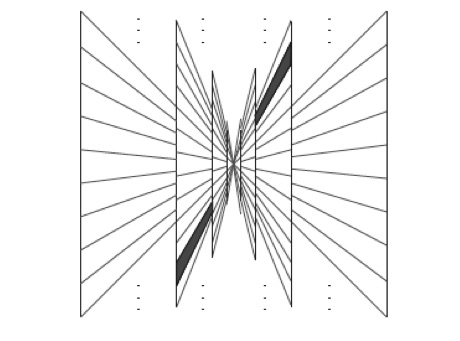
\includegraphics[width=0.4\textwidth]{../../Diagrams/tiling_nocone.jpg}
\end{figure}
\end{frame}

\begin{frame}
\begin{block}{Cone Adapted Shearlets}
For $\psi,\tilde{\psi},\phi\in L^2(\mathbb{R}^2)$ and $c\in \mathbb{Z}^2$ the \textbf{cone adapted shearlet system} is defined by 
$$
\mathcal{SH}(\phi,\psi,\tilde{\psi},c):=P_{\mathcal{R}}\Phi(\phi,c_1)\cup P_{\mathcal{C}_h}\Psi(\psi,c)\cup P_{\mathcal{C}_v}\tilde{\Psi}(\tilde{\psi},c)
$$
\end{block}
\begin{figure}[h!]
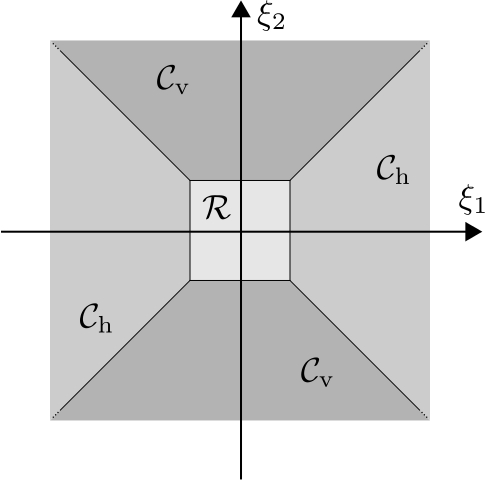
\includegraphics[width=0.5\textwidth]{../../Diagrams/cones.jpg}
\end{figure}
\end{frame}

\begin{frame}{Universal Shearlets and $0$-Shearlets}
\begin{block}{}
\begin{itemize}
\item Parabolic scaling is well suited to approximate functions with singularities over parabolic curves; we would like to inpaint the EPIs that have singularities over lines.
\pause
\item For more flexibility on the "level of anisotropy" of the functions that one would like to approximate, one can use a different scaling parameter in each scale (scaling sequence), $(\alpha_j)_{j\in I}\subseteq (-\infty,2)$, with associated scaling matrices 
$$
A_{j,\alpha_j} = \left( \begin{matrix} 2^j & 0 \\ 0 & 2^{\alpha_j j/2}\end{matrix}\right)
$$
\pause 
\item With $A_{j,\alpha_j}$ we can define the \textbf{Universal Shearlet System} (Kutyniok, Genzel, 2014), a generalization of the cone-adapted shearlet system for different level of anisotropy.
\end{itemize}
\end{block}
\end{frame}

\begin{frame}
\begin{block}{Schwartz Functions Space}
$$
\begin{aligned}
\mathbb{S}(\mathbb{R}^d):=\{\phi\in C^{\infty}(\mathbb{R}^d)&|\forall K,N\in\mathbb{N}_0:\\
&\sup_{x\in\mathbb{R}^d}(1+|x|^2)^{-N/2}\sum_{|\alpha|\leq K}|D^{\alpha}\phi(x)|<\infty\}
\end{aligned}
$$
\end{block}

\pause
\begin{block}{Meyer and Corona Scaling Functions}
Let $\phi\in\mathbb{S}(\mathbb{R})$ with $0\leq \hat{\phi}\leq 1$, $\hat{\phi}(u)=1$ for $u\in [-1/16,1/16]$ and $\text{supp}(\hat{\phi})\subset [-1/8,1/8]$; then $\phi$ is usally called \textbf{Meyer scaling function}. One can define then the \textbf{corona scaling function} for $j\in\mathbb{N}_0$ for $\xi = (\xi_1,\xi_2)\in \mathbb{R}^2$ by
$$
\begin{aligned}
\hat{\Phi}(\xi)&:= \hat{\phi}(\xi_1)\hat{\phi}(\xi_2)\\
W(\xi)&:= \sqrt{\hat{\Phi}^2(2^{-2}\xi)-\hat{\Phi}^2(\xi)}\\
W_j(\xi)&:= W(2^{-2j}\xi)
\end{aligned}
$$
The functions $W_j$ are compactly supported in corona-shaped scaling levels $\mathcal{K}_j:=[2^{-2j-1},2^{2j-1}]^2\setminus (-2^{2j-4},2^{2j-4})^2$.

\end{block}
\end{frame}

\begin{frame}
\begin{block}{Bump-like Function}
A \textbf{bump-like} function is defined as $v\in C^{\infty}(\mathbb{R})$ such that $\text{supp}(v)\subset[-1,1]$ and 
$$
\begin{aligned}
& |v(u-1)|^2+|v(u)|^2+|v(u+1)|^2 = 1 \quad \textrm{for} \quad u\in[-1,1] \quad \textrm{,and}\\
& v(0)=1 \quad \textrm{and} \quad v^{(n)}(0)=0\quad\textrm{for}\quad n\geq 1
\end{aligned}
$$
\end{block}
\begin{figure}[h!]
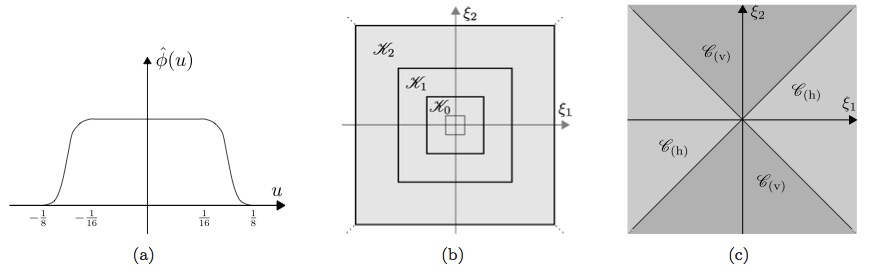
\includegraphics[width=\textwidth]{../../Diagrams/alphapartcones.jpg}
\end{figure}
\end{frame}

\begin{frame}
\begin{block}{Scaling and Shearing Matrices}
Let $j\in\mathbb{Z}$, $k\in\mathbb{N}$ and $\alpha_j\in (-\infty,2)$ for all $j\in\mathbb{Z}$, then
$$
A_{j,\alpha_j,(h)}:=\left(\begin{matrix} 2^j & 0 \\ 0 & 2^{\alpha_jj/2}\end{matrix}\right) \quad \textrm{,}\quad S_{k,(h)}:=\left(\begin{matrix} 1 & k\\ 0 & 1\end{matrix}\right)
$$
$$
A_{j,\alpha_j,(v)}:=\left(\begin{matrix}2^{\alpha_j j/2} & 0 \\ 0 & 2^j \end{matrix}\right)\quad \textrm{,}\quad S_{k,(v)}:=\left(\begin{matrix} 1 & 0 \\ 1 & k\end{matrix}\right)
$$
\end{block}
\bigskip
\pause
\begin{block}{Adapted Cone Functions}
Let $\iota\in\{h,v\}$ and $\xi=(\xi_1,\xi_2)\in\mathbb{R}^2$, then
$$
V_{(h)}(\xi):=v(\xi_2/\xi_1)\textrm{,}\quad V_{(v)}(\xi):=v(\xi_1/\xi_2)\textrm{,}\quad \xi\in\mathbb{R}^2.
$$
\end{block}
\end{frame}

\begin{frame}
\begin{block}{Ingredients for the Universal Shearlet System}
Let $\Phi$, $W$, $V_{(h)}$, $V_{(v)}\in L^2(\mathbb{R}^2)$ be defined as before.
\begin{enumerate}
\item[1.] \textbf{Coarse scaling functions}: For $k\in\mathbb{Z}^2$, we set 
$$
\psi_{-1,k}:=\Phi(x-k)\textrm{,}\quad x\in\mathbb{R}^2.
$$
\item[2.] \textbf{Interior shearlets}: Let $\alpha_j\in (-\infty,2)$, $j\in\mathbb{N}_0$, $k\in\mathbb{Z}$ with $|k|< 2^{(2-\alpha)j/2}$, $m\in\mathbb{Z}^2$ and $\iota\in\{h,v\}$. The shearlets will be given by 
\small
$$
\begin{aligned}
\hat{\psi}^{\alpha_j,(\iota)}_{j,k,m}(\xi):=2^{-(\alpha_j+2)j/4}W(2^{-j}\xi)&V_{(\iota)}(\xi^{\top} A_{-j,\alpha_j,(\iota)}S_{-k,(\iota)})\\
&e^{-2\pi i\xi^{\top}A_{-j,\alpha_j,(\iota)}S_{-k,(\iota)}}\textrm{,}\quad \xi\in\mathbb{R}^2
\end{aligned}
$$
\end{enumerate}
\end{block}
\end{frame}

\begin{frame}
\begin{block}{}
\begin{enumerate}
\item[3.] \textbf{Boundary shearlets}: For $\alpha_j \in(-\infty,2)$, $j\geq 1$, $k=\pm\lceil 2^{(2-\alpha_j)j/2}\rceil$ and $k\in\mathbb{Z}^2$, we define
$$
\hat{\psi}_{j,k,m}^{\alpha_j}:=
\begin{cases}
2^{-(\alpha_j+2)j/4-1/4}&W(2^{-j}\xi)V_{(h)}(\xi^{\top} A_{-j,\alpha_j,(h)}S_{-k,(\iota)})\\
&e^{-\pi i\xi^{\top}A_{-j,\alpha_j,(h)}S_{-k,(h)}m}\textrm{,}\quad \xi\in\mathcal{C}_{(h)},\\
2^{-(\alpha_j+2)j/4-1/4}&W(2^{j}\xi)V_{(v)}(\xi^{\top}A_{-j,\alpha_j,(v)}S_{-k,(v)})\\
&e^{-\pi i\xi^{\top}A_{-j,\alpha_j,(v)}S_{-k,(h)}m}\textrm{,}\quad \xi\in\mathcal{C}_{(v)}
\end{cases}
$$
and in the case $j=0$, $k=\pm 1$, we define
$$
\hat{\psi}^{\alpha_j}_{0,k,m}:=
\begin{cases}
W(\xi) V_{(h)}(\xi^{\top}S_{-k,(h)})e^{-2\pi i\xi^{\top}m}\textrm{,}\quad \xi\in\mathcal{C}_{(h)}\textrm{,}\\
W(\xi)V_{(v)}(\xi^{\top}S_{-k,(v)})e^{-2\pi i\xi^{\top}m}\textrm{,}\quad \xi\in\mathcal{C}_{(v)}.
\end{cases}
$$
\end{enumerate}
\end{block}

\pause
\begin{block}{Scaling Sequence}
A sequence $(\alpha_j)_{j\in\mathbb{N}_0}\subset \mathbb{R}$ is called a scaling sequence if
$$
\alpha_j\in A_j:=\{2n/j| n\in\mathbb{Z},n\leq j-1\}=\{\ldots,-4/j,-2/j,0,2/j,\ldots,2-2/j\}
$$
\end{block}
\end{frame}

\begin{frame}
\begin{block}{Universal Shearlet System}
Let $(\alpha_j)_{j\in \mathbb{N}_0}$ be a scaling sequence, $\phi$ a Meyer scaling function and $v$ a bump-like function, then \textbf{the universal shearlet system} is given by
$$
\mathcal{SH}(\phi,v,(\alpha_j)_j):=\mathcal{SH}_{\text{Low}}(\phi)\cup\mathcal{SH}_{\text{Int}}(\phi,v,(\alpha_j)_j)\cup\mathcal{SH}_{\text{Bound}}(\phi,v,(\alpha_j)_j),
$$
where
$$
\begin{aligned}
\mathcal{SH}_{\text{Low}}(\phi)&:=\{\psi_{-1,m}|m\in\mathbb{Z}^2\}\\
\mathcal{SH}_{\text{Int}}(\phi,v,(\alpha_j)_j)&:=\{\psi_{j,k,m}^{\alpha_j,(\iota)}|j\geq 0,|k|< 2^{(2-\alpha_j)j/2},m\in\mathbb{Z}^2,\iota\in\{h,v\}\},\\
\mathcal{SH}_{\text{Bound}}(\phi,v,(\alpha_j)_j)&:=\{\psi_{j,k,m}^{\alpha_j}|j\geq 0,|k|=\pm 2^{(2-\alpha_j)j/2},m\in\mathbb{Z}^2\}.
\end{aligned}
$$
\end{block}

\begin{block}{Parseval Frame Property}
If $(\alpha_j)_j$ is a scaling squence then $\mathcal{SH}(\phi,v,(\alpha_j)_j)$ is a Parseval frame for $L^2(\mathbb{R}^2)$.
\end{block}
\end{frame}

\begin{frame}
\begin{block}{$0$-Shearlets System}
The $0$-Shearlets System are obtained by selecting the scaling sequence $(\alpha_j)_{j\in\mathbb{Z}}=(-2/j)_{j\in\mathbb{Z}}$ on the Universal Shearlets System; they are sensible to linear singularities and have an associated scaling matrix given by
$$
A_j =\left(\begin{matrix} 2^j & 0 \\ 0 & 2^{-1} \end{matrix}\right)
$$
We used the $0$-Shearlets System as the selected sparsifying system for the sparse EPIs inpainting.
\end{block}
\end{frame}

\begin{frame}{Shearlet-based inpainting with iterative hard thresholding}
\small
\begin{algorithm}
    \SetKwInOut{Input}{Input}
    \SetKwInOut{Output}{Output}
		\SetKwInOut{Compute}{Compute}

    \Input{Sparse EPI $y$, sampling matrix $M$, $\delta_{init}$,$\delta_{min}$, iterations}
		\Compute{$x_0:=0$;\\
						 $\delta_0:=\delta_{init}$;\\
						 $\lambda:=(\delta_{min})^{1/(iterations-1)}$;\\
						 $\Gamma_0 := \textrm{supp}(T(x_0))$;\\
					   $\beta_0 := T_{\Gamma_0}(y-Mx_0)$;\\
						 $\alpha_0 =\frac{||\beta_0||_2^2}{||MT^*(\beta_0)||_2^2}$;\\
						 \textbf{for} $n:=0$ \textbf{to} (iterations-1) \textbf{do}\\
							 \hspace{5mm} $x_{n+1}=T^*(Thr_{\delta_n}(T(x_n+\alpha_n(y-Mx_n))))$;\\
							 \hspace{5mm} $\Gamma_{n+1} := \textrm{supp}(T(x_{n+1}))$;\\
					     \hspace{5mm} $\beta_{n+1} := T_{\Gamma_{n+1}}(y-Mx_{n+1})$;\\
						 	 \hspace{5mm} $\alpha_{n+1}: =\frac{||\beta_{n+1}||_2^2}{||MT^*(\beta_{n+1})||}$;\\
							 \hspace{5mm} $\delta_{n+1} :=\lambda\delta_n;$\\
							\textbf{end}}
    \Output{Inpainted EPI $x_{iterations}$}
\end{algorithm}
\normalsize
\end{frame}

\begin{frame}{Results on EPIs inpainting}
\begin{figure}[!tbp]
  \centering
  \begin{minipage}[b]{0.40\textwidth}
    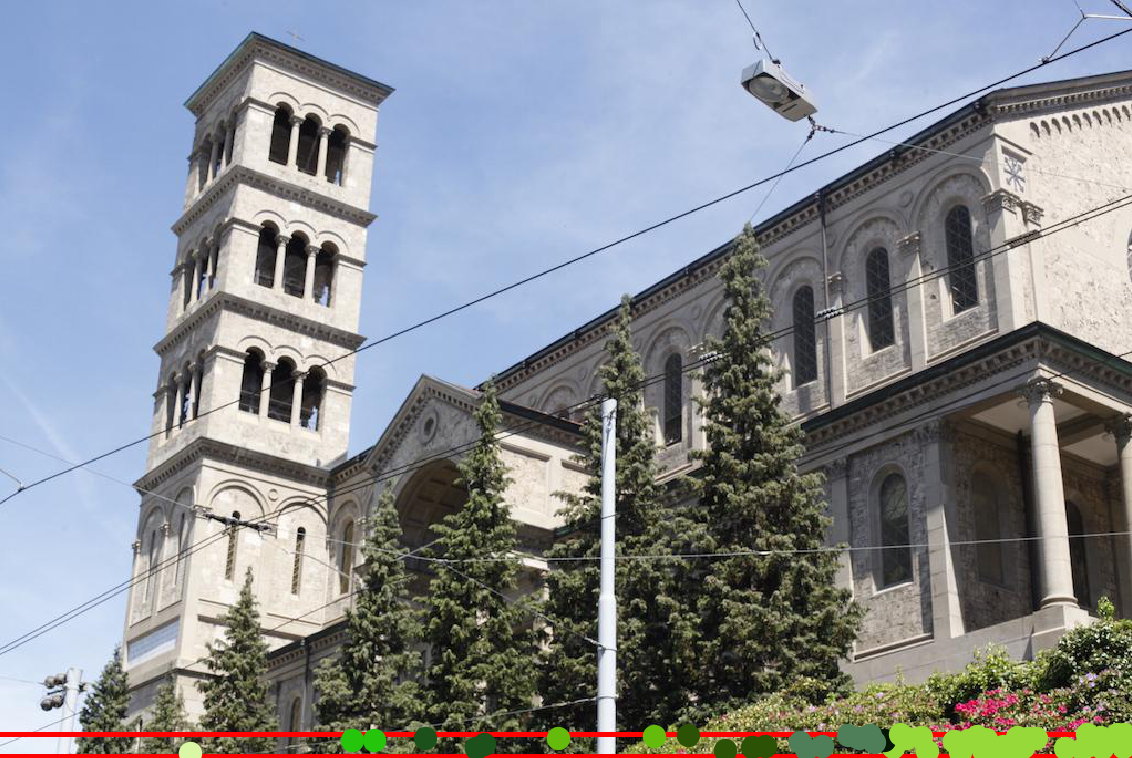
\includegraphics[width=\textwidth]{../../Diagrams/results/EPIs/673_10_102_4_48_8_strip.png}
  \end{minipage}
	\pause
 % \hfill
  \begin{minipage}[b]{0.40\textwidth}
    
\includegraphics[width=\textwidth]{../../Diagrams/results/EPIs/673_10_102_7_48_8_dense.png}
  \end{minipage}
\end{figure}
\pause

\begin{figure}[!tbp]
  \centering
  \begin{minipage}[b]{0.40\textwidth}
    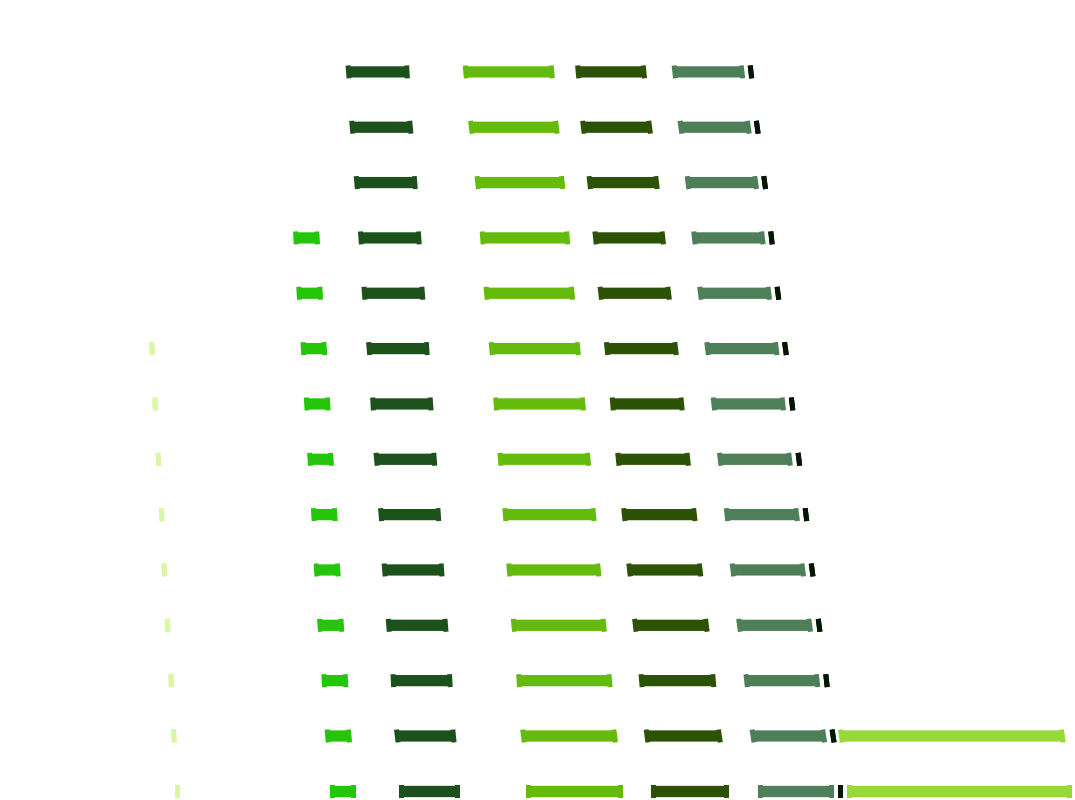
\includegraphics[width=\textwidth]{../../Diagrams/results/EPIs/673_10_102_7_48_8_sparse.png}
  \end{minipage}
	\pause
 % \hfill
  \begin{minipage}[b]{0.40\textwidth}
    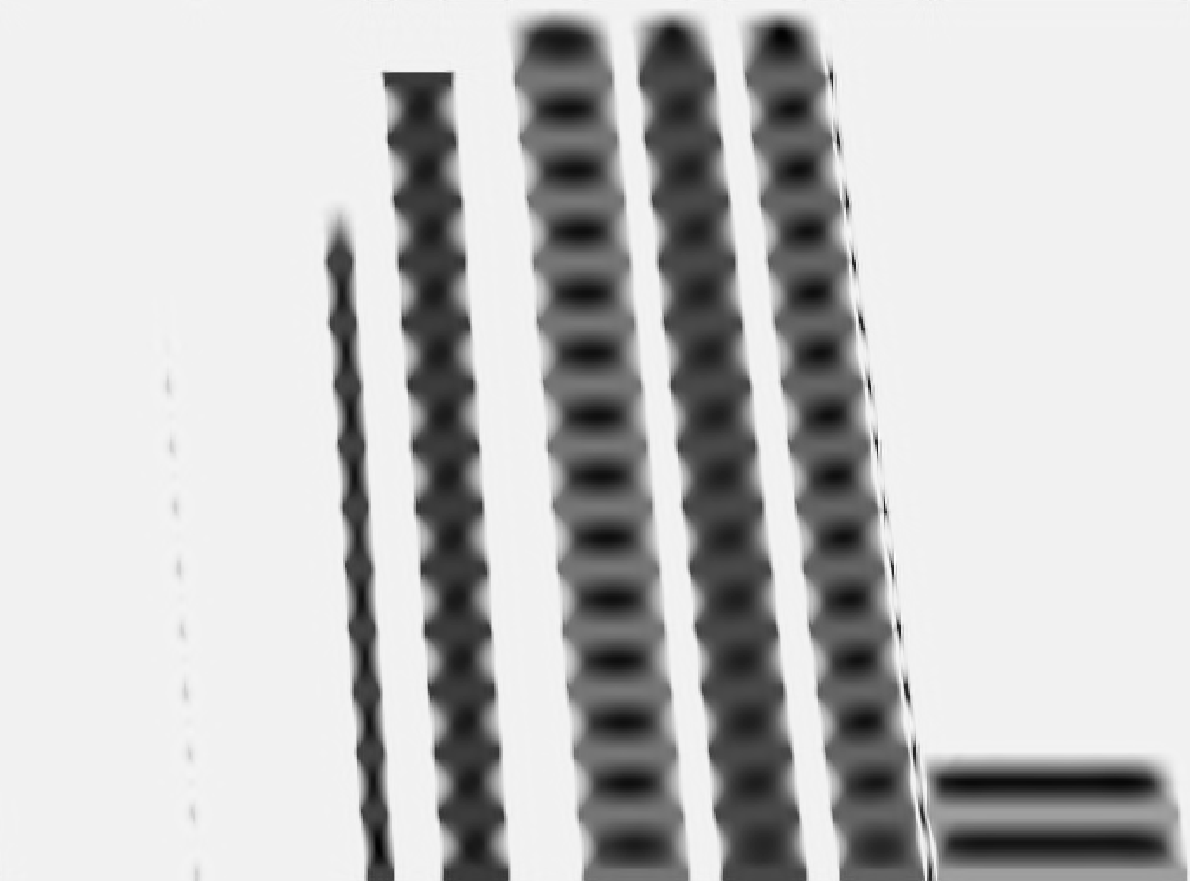
\includegraphics[width=\textwidth]{../../Diagrams/results/Inpainted/673_10_102_7_48_8_inpainted.png}
  \end{minipage}
\end{figure}

\end{frame}

\begin{frame}{Results on line detection and depth map estimation}
\begin{figure}[!tbp]
  \centering
  \begin{minipage}[b]{0.40\textwidth}
    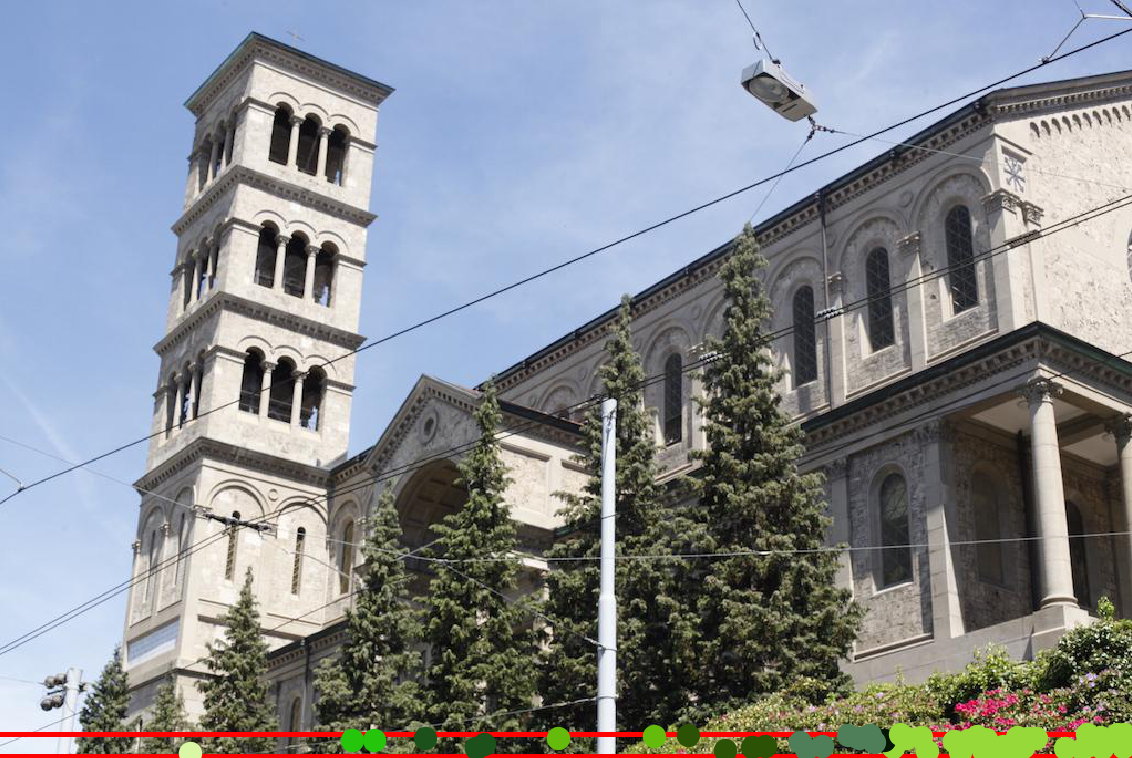
\includegraphics[width=\textwidth]{../../Diagrams/results/EPIs/673_10_102_4_48_8_strip.png}
  \end{minipage}
	\pause
 % \hfill
  \begin{minipage}[b]{0.40\textwidth}
    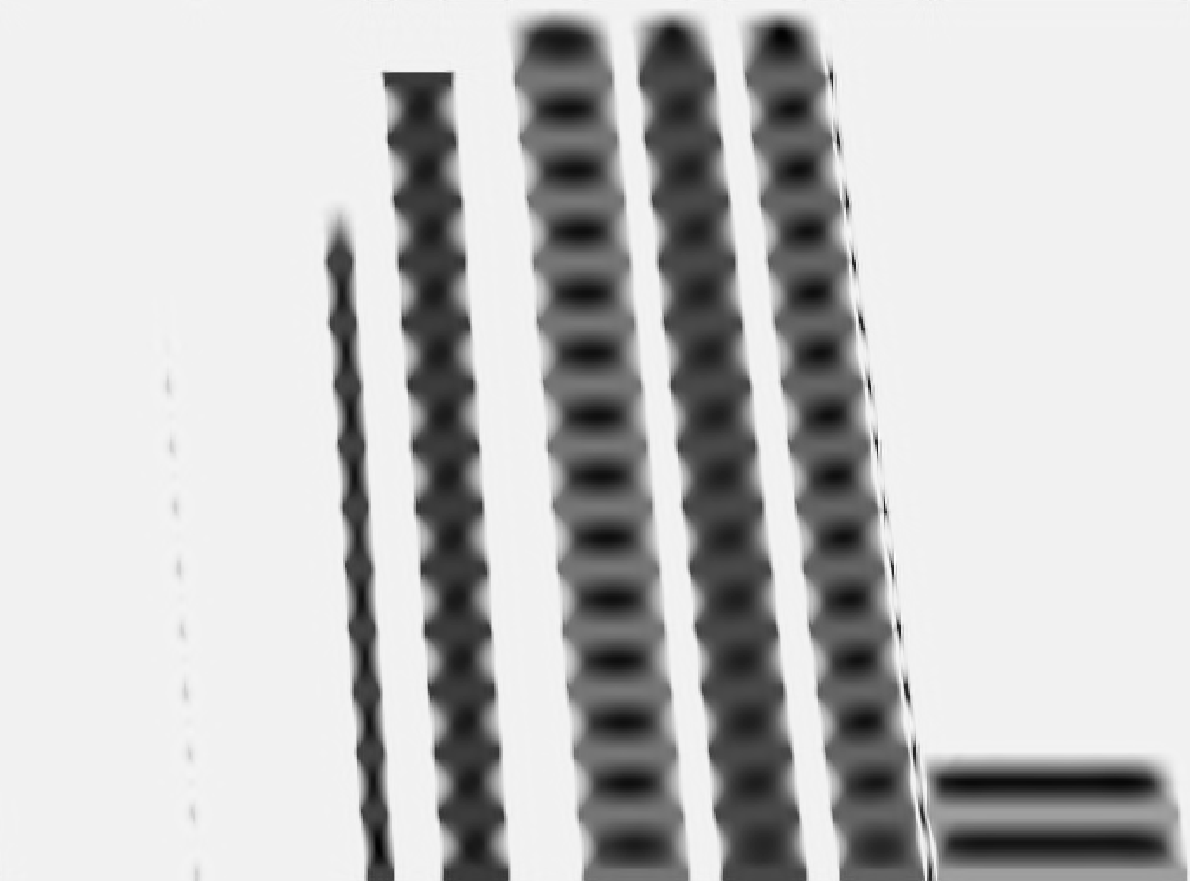
\includegraphics[width=\textwidth]{../../Diagrams/results/Inpainted/673_10_102_7_48_8_inpainted.png}
  \end{minipage}
\end{figure}
\pause

\begin{figure}[!tbp]
  \centering
  \begin{minipage}[b]{0.40\textwidth}
    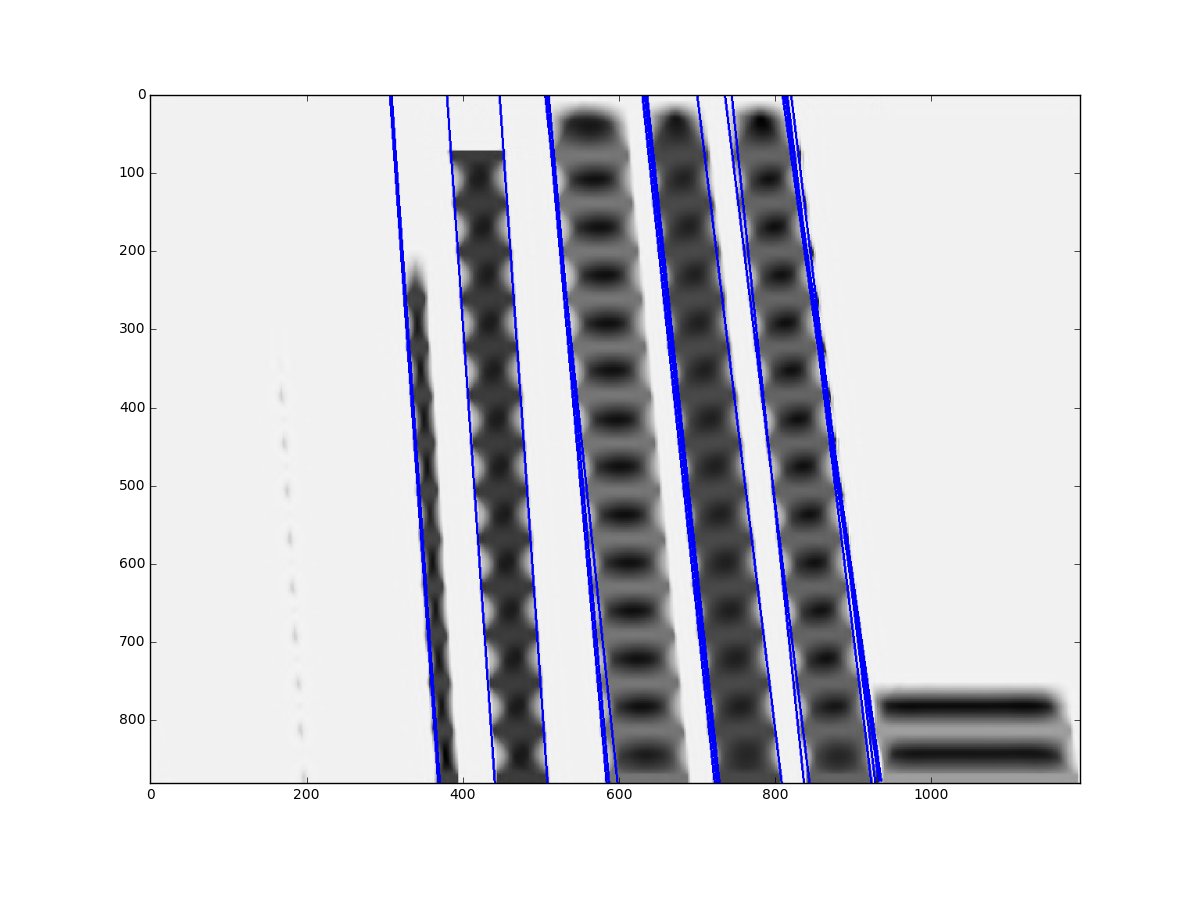
\includegraphics[width=\textwidth]{../../Diagrams/results/Disparity_benchmark/673_10_102_7_48_8_lines.png}
  \end{minipage}
	\pause
 % \hfill
  \begin{minipage}[b]{0.40\textwidth}
    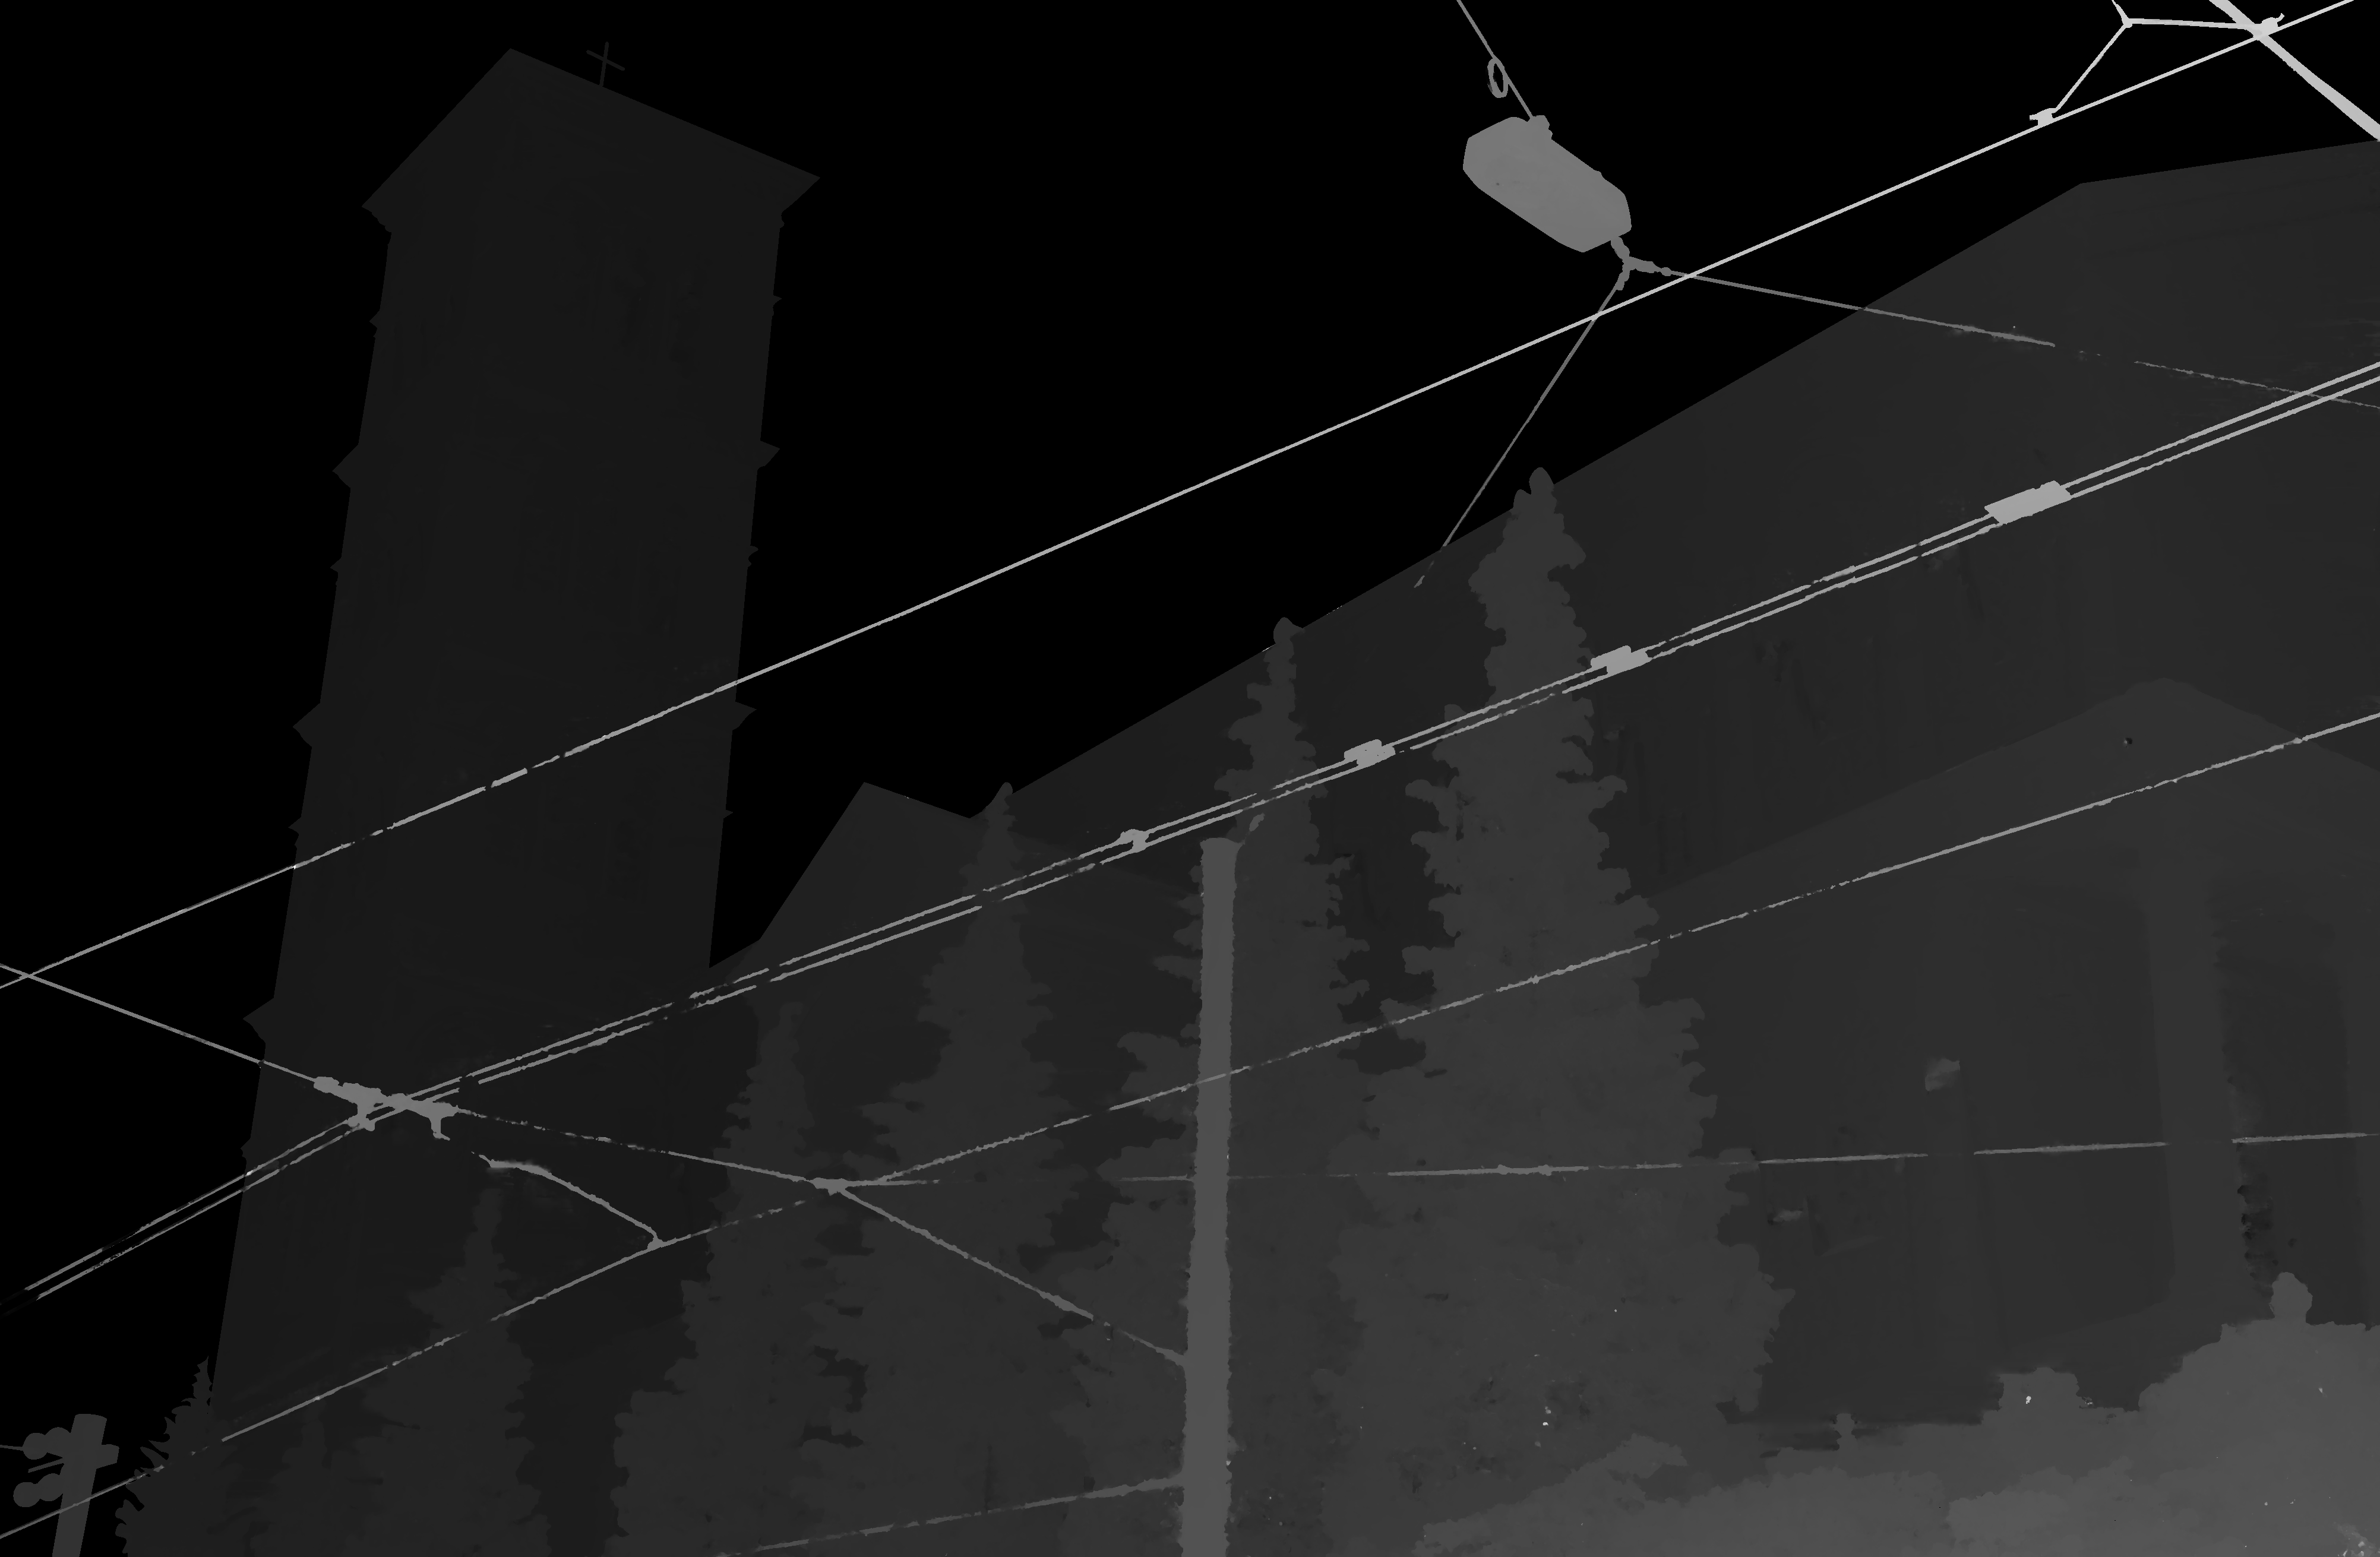
\includegraphics[width=\textwidth]{../../Diagrams/church_depth_0034.png}
  \end{minipage}
\end{figure}
\end{frame}

\begin{frame}
\begin{center}
\textbf{\huge{Conclusions and Outlook}}
\end{center}
\end{frame}

\begin{frame}{Thanks!}
\begin{center}
\Large{Questions?}
\end{center}
\begin{figure}[h!]
\centering
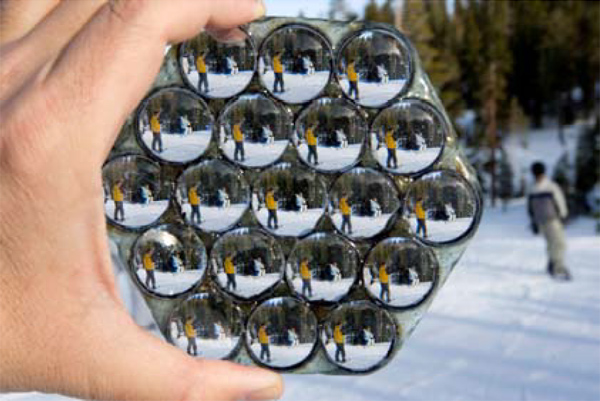
\includegraphics[width=0.8\textwidth]{./Images/lf-camera.jpg}
\end{figure}
\end{frame}

